\documentclass[a4paper]{article}

%% Language and font encodings
\usepackage[english]{babel}
\usepackage{graphicx}
\usepackage[T1]{fontenc}
\usepackage[utf8]{inputenc}

%% Sets page size and margins
\usepackage[a4paper,top=3cm,bottom=3cm,left=3cm,right=3cm,marginparwidth=1.75cm]{geometry}

\title{Concorrência e Paralelismo \\
\large Projecto 1}

\author{Didier Dias N45777\and Daniel Pimenta N45404}

\begin{document}
\maketitle

\begin{abstract}
O problema principal que foi resolvido foi a paralelização de um programa que simula um jogo de reversi, fornecido pelo professor. \\
Para tal foi utilizada a técnologia Cilk+ que nos permite facilmente criar threads que executam código em paralelo, podendo assim o computador utilizar vários cores para realizar o processamento do programa.\\
Foi nos possível realizar esta paralelização o que, se o tamanho do tabuleiro utilizado na simulação for relativamente elevado, diminui bastante o tempo de execução do programa.
\end{abstract}

\section{Introdução}


Foi-nos fornecido um programa em C que simula um jogo de reversi, estando este implementado iterativamente. O problema consiste em tentar paralelizar esse código, fazendo as alterações necessárias para esse efeito. Foram também feitas algumas otimizações de modo a que o programa corra o mais rapidamente possível, sem sacrificar a estabilidade do mesmo.\\
Para poder efetuar estas mudanças é preciso saber quais são as partes do código que podem ser paralelizadas, ou seja, partes que não entrem em conflito seja ao alterar a mesma posição de memória ao mesmo tempo ou mesmo manter a ordem dos métodos, no caso em que esta seja necessária.

\section{Método}
A função mais necessitada de paralelização é a make\textunderscore move visto que é o local onde ocorre a grande parte do tempo de execução do programa, onde são encontrados todos os movimentos possíveis num dado momento e de seguida verificar qual destes o que o jogador deveria escolher para maximizar a sua pontuação. Para paralelizar a obtenção de todos os moves possíveis o trabalho foi dividido por linhas, ou seja, utilizamos um cilk\textunderscore for para cada linha da matriz do tabuleiro de modo a verificar se seria permitida uma jogada nessa mesma posição. Este trabalho poderia ser dividido ainda mais, criando um job para cada posição do tabuleiro no entanto, depois da realização de alguns testes, verificámos que esse tipo de distribuição iria abrandar a execução do programa, visto que a carga de trabalho dentro de cada um seria mínima comparada com a carga necessária para criar um número de workers tão elevado.
De modo a que cada processo guardasse os seus resultados sem entrar em conflito foi criada uma matriz para guardar os dados de cada movimento.

O outro local onde a paralelização faz sentido, neste programa, seria na procura da melhor jogada possível, de entre todas as possíveis. Para tal foi aplicada uma metodologia semelhante à utilizada anteriormente, na qual é criado um job para cada linha da matriz de movimentos aplicáveis. Desta maneira, cada thread irá tratar de verificar qual a jogada que trará mais ganhos ao utilizador de entre uma subparte da matriz total. De seguida estes serão comparados entre de modo a obter o melhor de todos. Esta paralelização não diminui tanto o tempo de execução como a anterior, visto que os cálculos executados dentro desta são menores que na obtenção dos movimentos possíveis.

Foram realizados vários testes sobre se seria oportuno paralelizar outras partes do código, no entanto em nenhuma delas seriam obtidos ganhos significativos o suficiente para a justificar. Um desses casos seria o cálculo das pontuações finais. No entanto este método apenas vai a cada posição do tabuleiro e verifica qual foi o jogador que colocou uma peça nesta posição. Neste caso não haveriam ganhos suficientes para paralelizar esta implementação visto que a o código executado é mínimo comparado com o necessário para a criação dos workers, a não ser que o board seja bastante grande, altura em que o programa iria crashar por falta de resources, tentando executar as outras partes do código.

O padrão de paralelização utilizado foi o Reducer visto que o problema inicial, uma matriz, foi reduzido às suas várias linhas sendo criado um job para cada uma delas. Após todos os workers terem terminado o seu trabalho é feita a redução de modo a obter o resultado final a partir do resultado individual de cada um.   

\section{Validação}
De modo a verificar se o programa irá correr sem problemas foram realizados bastantes testes em diferentes máquinas utilizando flags e inputs diferentes, de modo a tentar testar todos os casos possíveis no qual o programa poderia ser executado.
Isto para um programa implementado sequencialmente talvez seria o suficiente para garantir um elevado nível de confiança no programa. No entanto, visto que este é executado em paralelo não existe uma certeza da ordem de execução de cada um dos threads. Logo podem existir casos onde um thread se pode atrasar relativamente a outro, devido a ruido existente durante a execução do código. Para poder testar estas ocasiões seria necessário utilizar um "noise injector" de modo a poder simular um ambiente mais real, visto que seria alterada a ordem de finalização de cada thread.

Outra maneira de confirmar a integridade do código é verificando se não existe nenhum thread que aceda a mesma posição de memória que outro thread que possa possivelmente utilizar esses mesmos dados, tendo cada um as suas próprias variáveis ou esperando que os threads acabem de executar e fazer as suas alterações, caso seja necessário utilizar esses dados posteriormente.

\section{Avaliação}
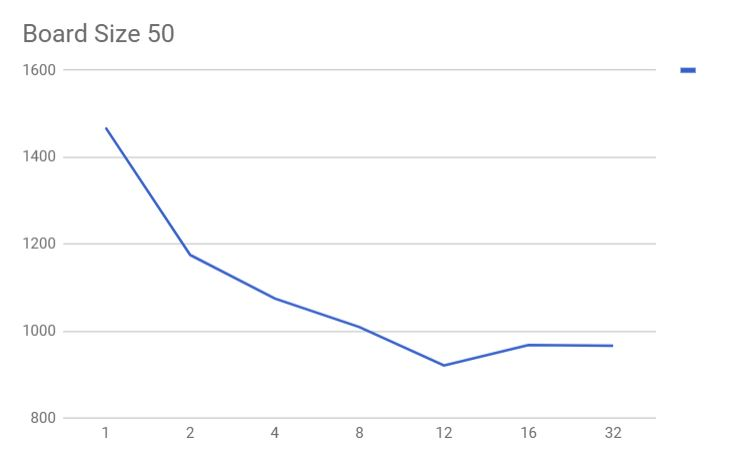
\includegraphics{bs50.JPG}
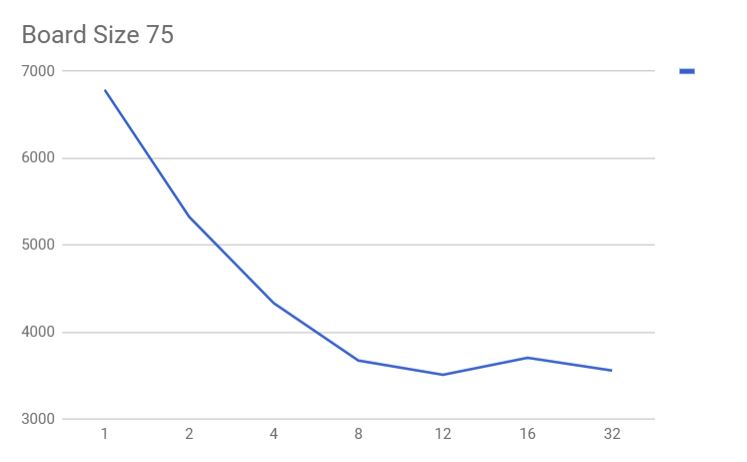
\includegraphics{bs75.JPG}
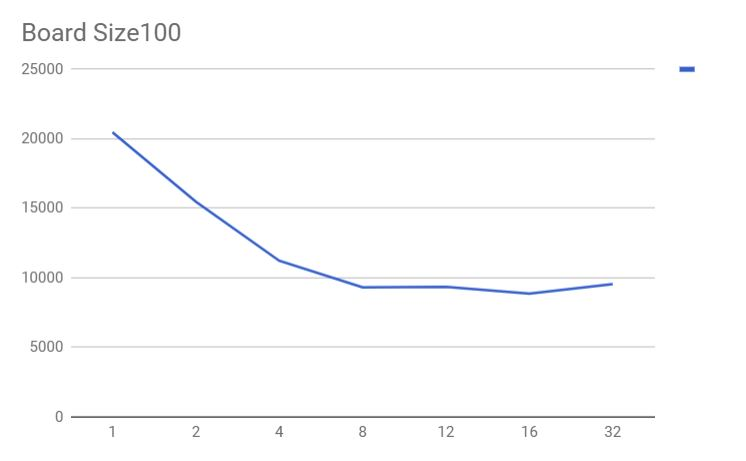
\includegraphics{bs100.JPG}

Os dados referentes às imagens acima foram obtidos através de vários testes na máquina de 16 cores, sendo que foi utilizada a média desses valores para simplificar a visualização dos mesmos tal como eliminar qualquer ruído durante a execução dos testes, possivelmente criado por outros alunos a realizar os seus testes.

Como se pode ver nos gráficos apresentados acima houve um aumento de velocidade bastante substancial na execução do código utilizando apenas 1 core contra utilizando múltiplos cores, tal como esperado, visto que foi feita a paralelização do programa tendo em conta o tempo de execução do mesmo.

Podemos também verificar que os maiores ganhos ocorrem utilizando 12 cores, com um tamanho de tabuleiro menos grande. Isto deve-se ao facto de que a quantidade de código executada por cada um dos processadores nesses jogos mais pequenos não justifica a criação de mais threads, levando mesmo a algum decréscimo de velocidade. 

O ganho de velocidade depende do tamanho do tabuleiro inicial sendo que quanto maior este for, mais eficiente será a paralelização. Isto pode ser explicado, como o ponto anterior, pela quantidade de carga que cada processador irá tratar. Outro fator que contribui para esse facto será que ao aumentar o tamanho do board, a parte paralelizada do programa irá crescer a uma velocidade superior superior ao troço de código iterativo ou seja, quanto maior o board, menos impacto terá a parte não paralelizada no tempo que o programa demora a executar, levando assim a mais ganhos.

\section{Conclusões}
Com este projeto foi concluido que paralelizar um programa é mais complicado que simplesmente criar um thread para tudo. Isto deve-se ao facto de ser necessário verificar se irá existir algum aumento de velocidade ou mesmo se haverá algum problema, nomeadamente "race conditions", a diferentes processos tentarem aceder à mesma posição de memória e o programa terminar, ou mesmo porque pode ser necessário manter a ordem de execução do programa. 
Foi também visível que a partir de um certo ponto, dado um problema de um tamanho fixo, não serve de muito aumentar o número de "cores" a utilizar pelo programa, visto que estes não irão aumentar a sua velocidade de execução, podendo mesmo levar a uma diminuição de performance.  

\section{Acknowledgments}
\begin{itemize}
\item André Neves - Nº46264
\begin{itemize}
\item Discussão sobre várias maneiras de implementar a paralelização, nomeadamente se seria melhor recursivamente ou iterativamente e sobre os vários padrões de paralelização e sobre qual o mais correto para esta situação.
\end{itemize}
\item Daniel Henriques - Nº46144
\begin{itemize}
\item Realização de testes para verificar quais as operações que valem a pena ser optimizadas, tendo em conta a complexidade e número de operações.
\end{itemize}

\end{itemize}

\section{Bibliografia}
\begin{itemize}
\item Stack Overflow
\end{itemize}

\end{document}

